To further motivate a BDT-based analysis, an alternative final selection derived from a 3-D optimization (similar to that used in Ref.~\cite{CMSLQ2_2016}) was studied. MC samples correspond to those listed in Section~\ref{sec:Samples} but are stored in the NanoAOD v6 format. The preselection, MC corrections, background normalization, and b-jet tag requirements described in Sections~\ref{sec:EventSelection}--\ref{sec:Backgrounds} were applied. 

To separate signal from background, a 3-D scan of thresholds over the kinematic variables \ST, \Muu, and \MujTwo was performed on 2016 simulation, while maximizing the Punzi significance for each leptoquark mass hypothesis. Any volitility or plateaus in the optimized thresholds introduced by sparse background MC statistics were smoothed out by fitting a quadratic to the points. To constrain the fit to a monotonically increasing function, a cutoff to the thresholds was applied approximately where they no longer increased, and a re-fit of the points below the cuttoff was performed. For leptoquark hypotheses with masses above the cutoff, the thresholds were kept constant. Figure~\ref{figapp:quadraticfits} shows the optimized thresholds and the quadratic fits before and after the cutoff was applied. The final set of cuts on each variable were extracted from the fit at each leptoquark hypothesis mass, as shown in Fig.~\ref{figapp:3doptimizedcuts}.

\begin{figure}[H]
    \centering
    {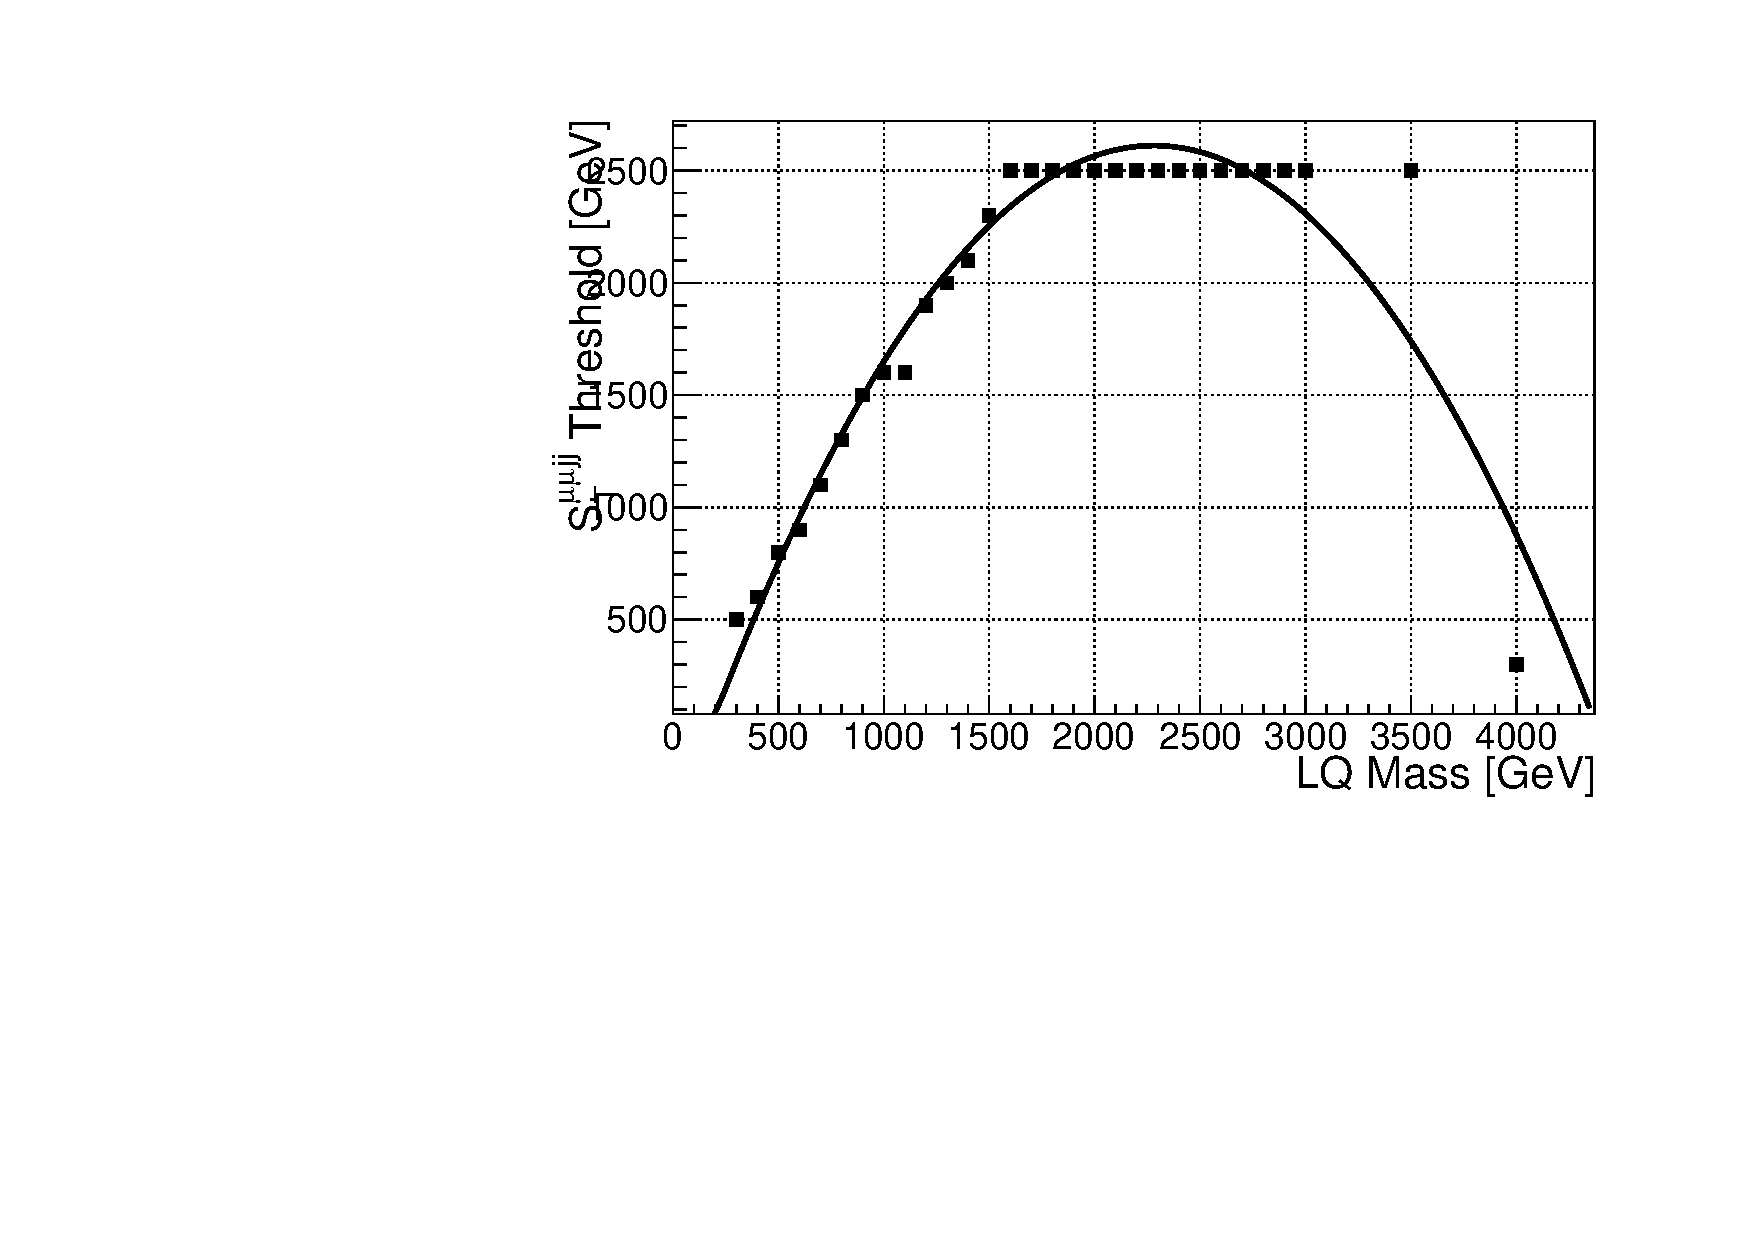
\includegraphics[width=.32\textwidth]{Images/Analysis/Results_Testing_2016_stockNanoAODv6/OptimizationLQ_uujj_St_uujj_pol2.pdf}}
    {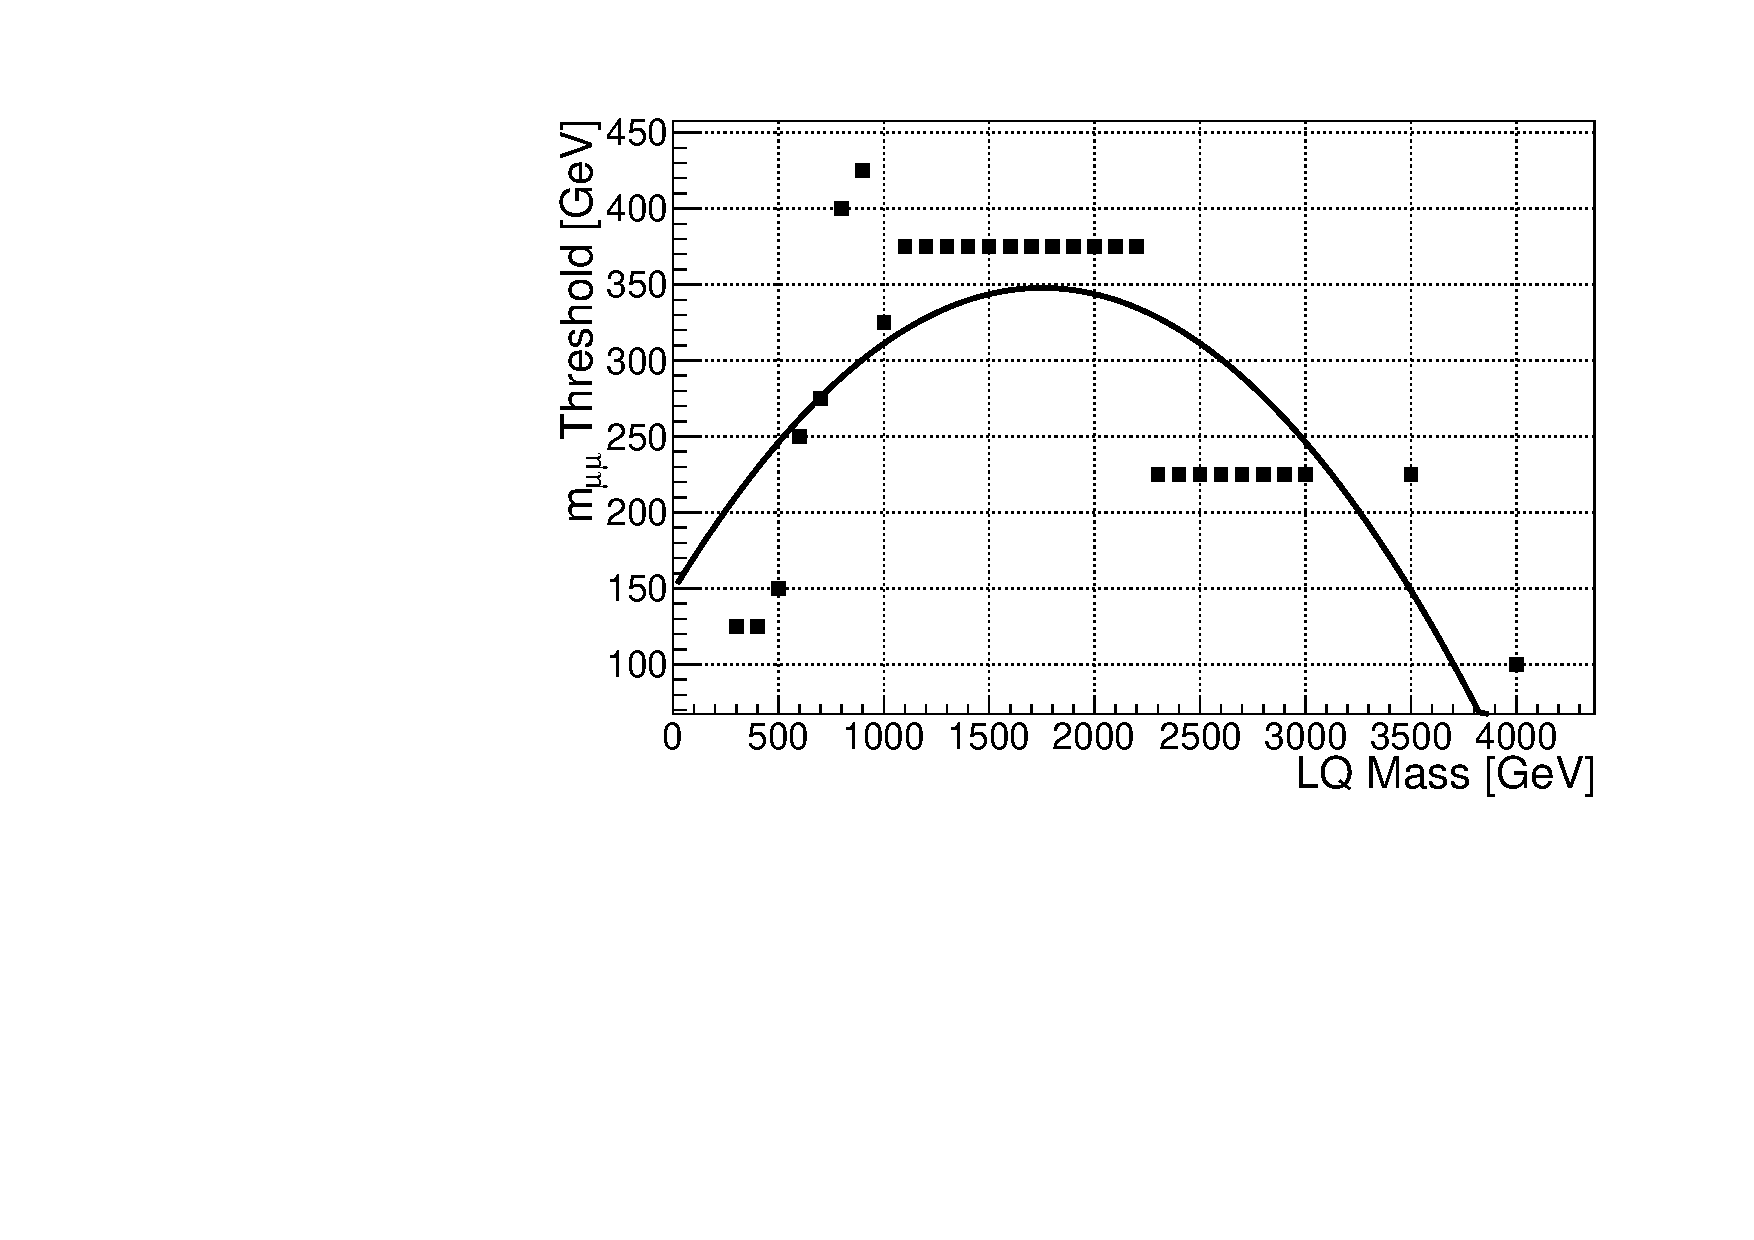
\includegraphics[width=.32\textwidth]{Images/Analysis/Results_Testing_2016_stockNanoAODv6/OptimizationLQ_uujj_M_uu_pol2.pdf}}
    {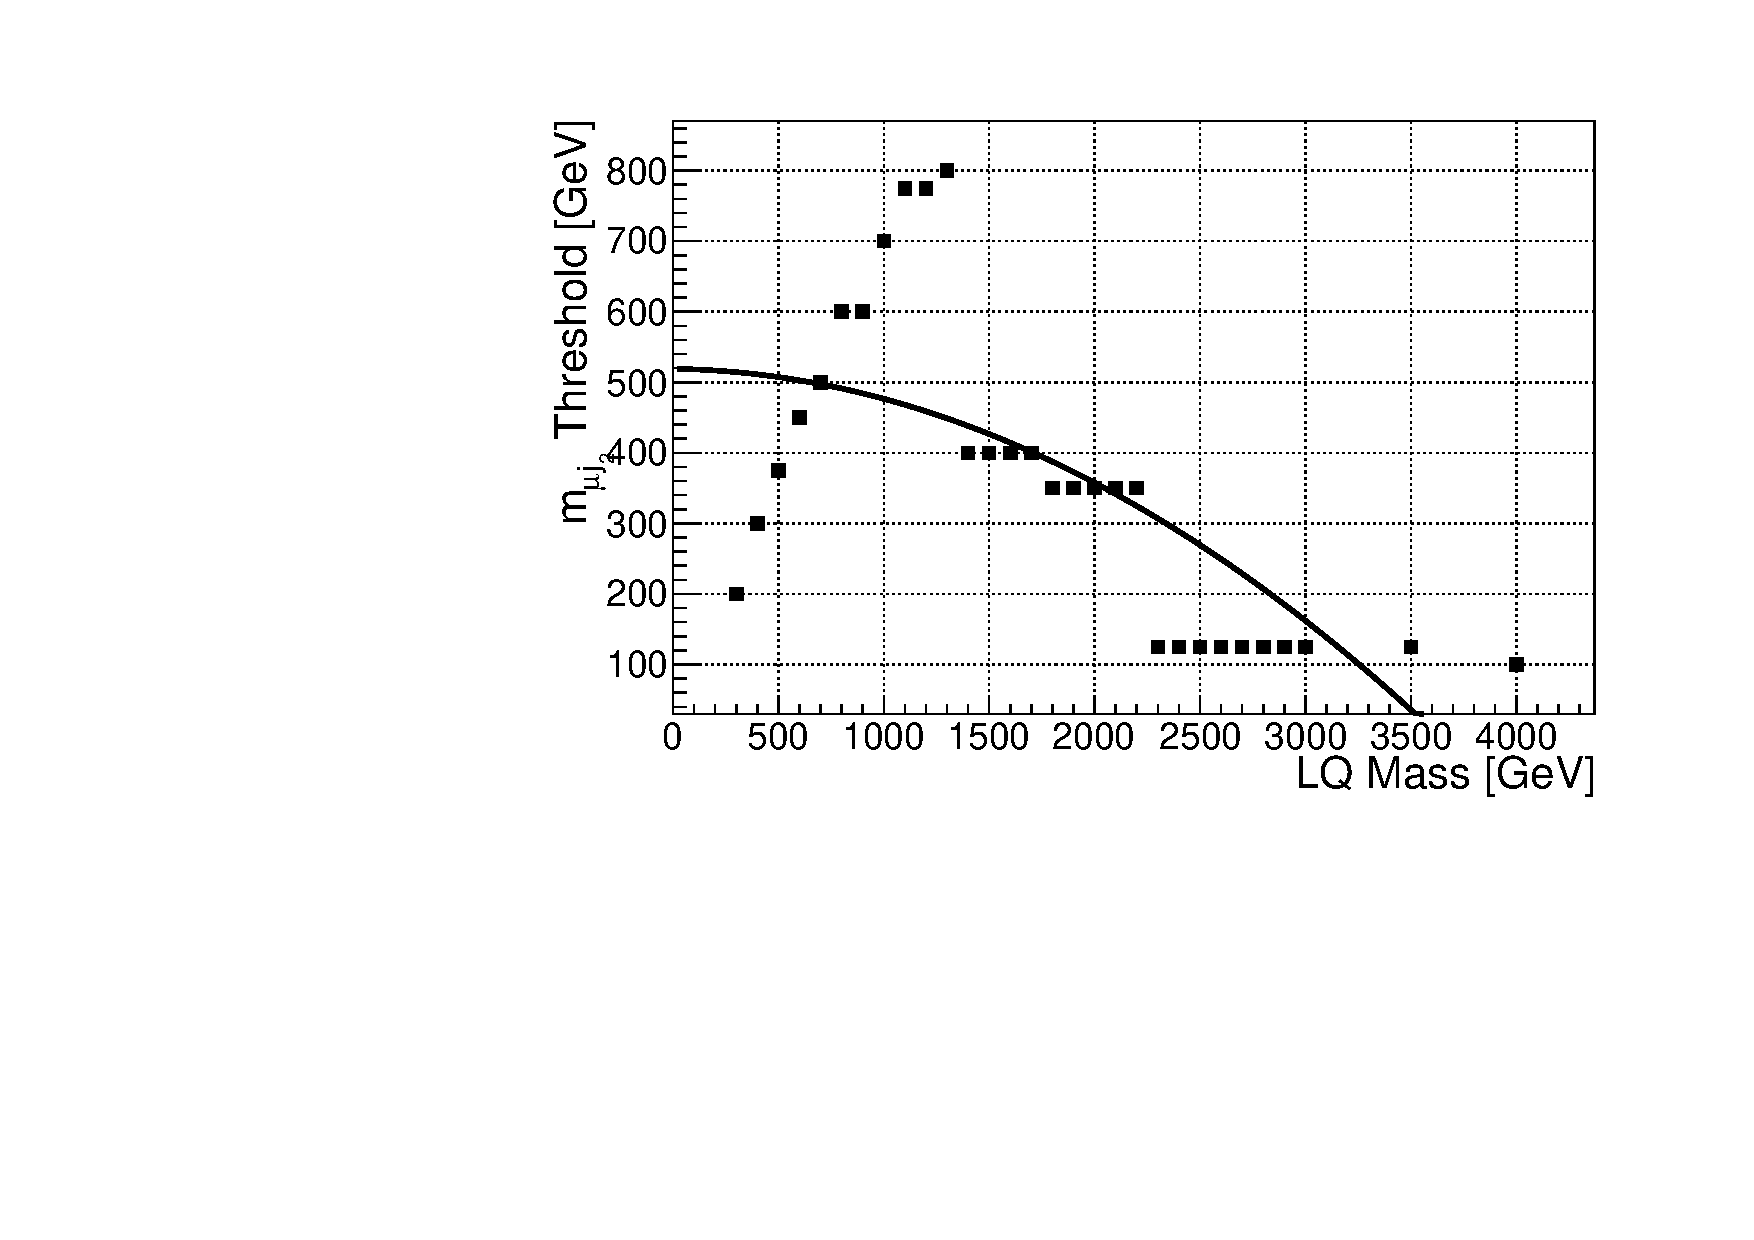
\includegraphics[width=.32\textwidth]{Images/Analysis/Results_Testing_2016_stockNanoAODv6/OptimizationLQ_uujj_M_uujj2_pol2.pdf}}
    {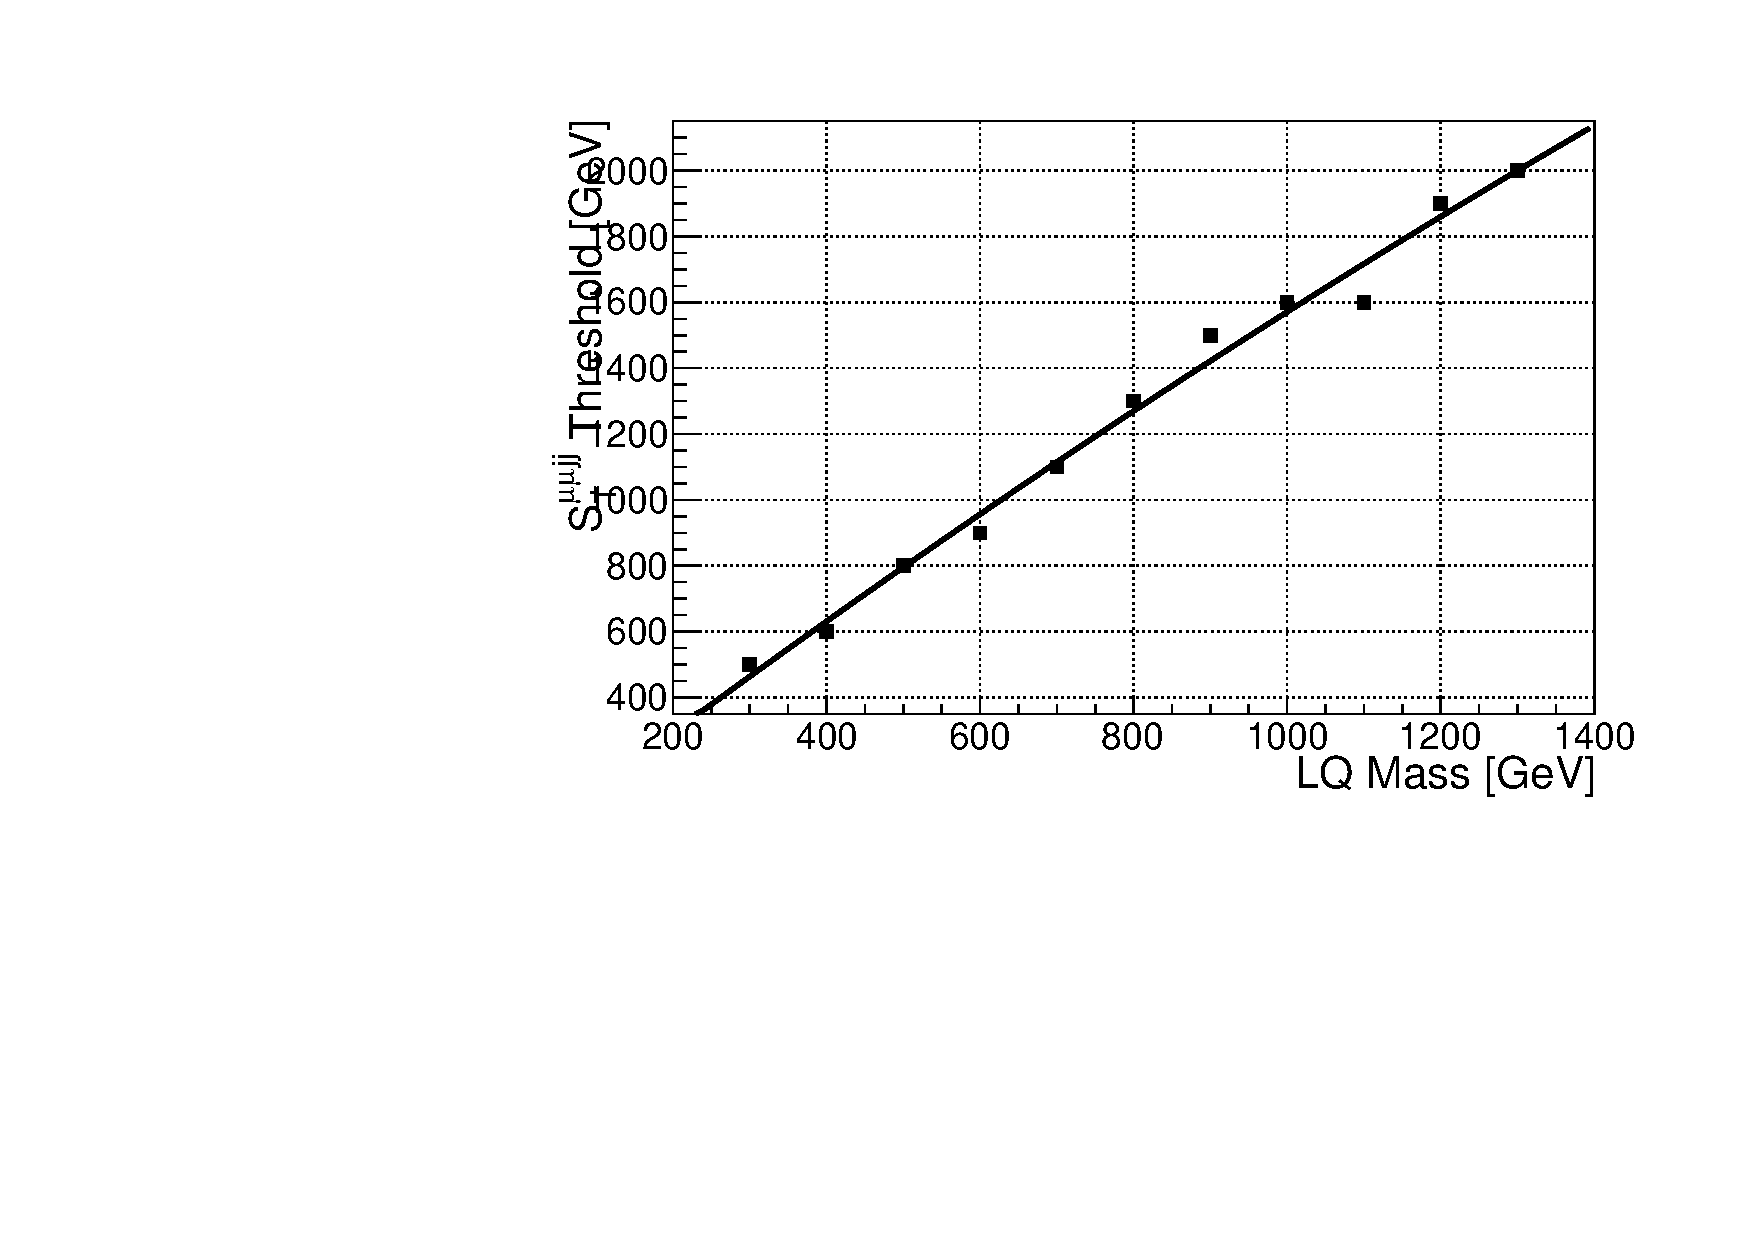
\includegraphics[width=.32\textwidth]{Images/Analysis/Results_Testing_2016_stockNanoAODv6/OptimizationLQ_uujj_St_uujj_pol2cutoff.pdf}}
    {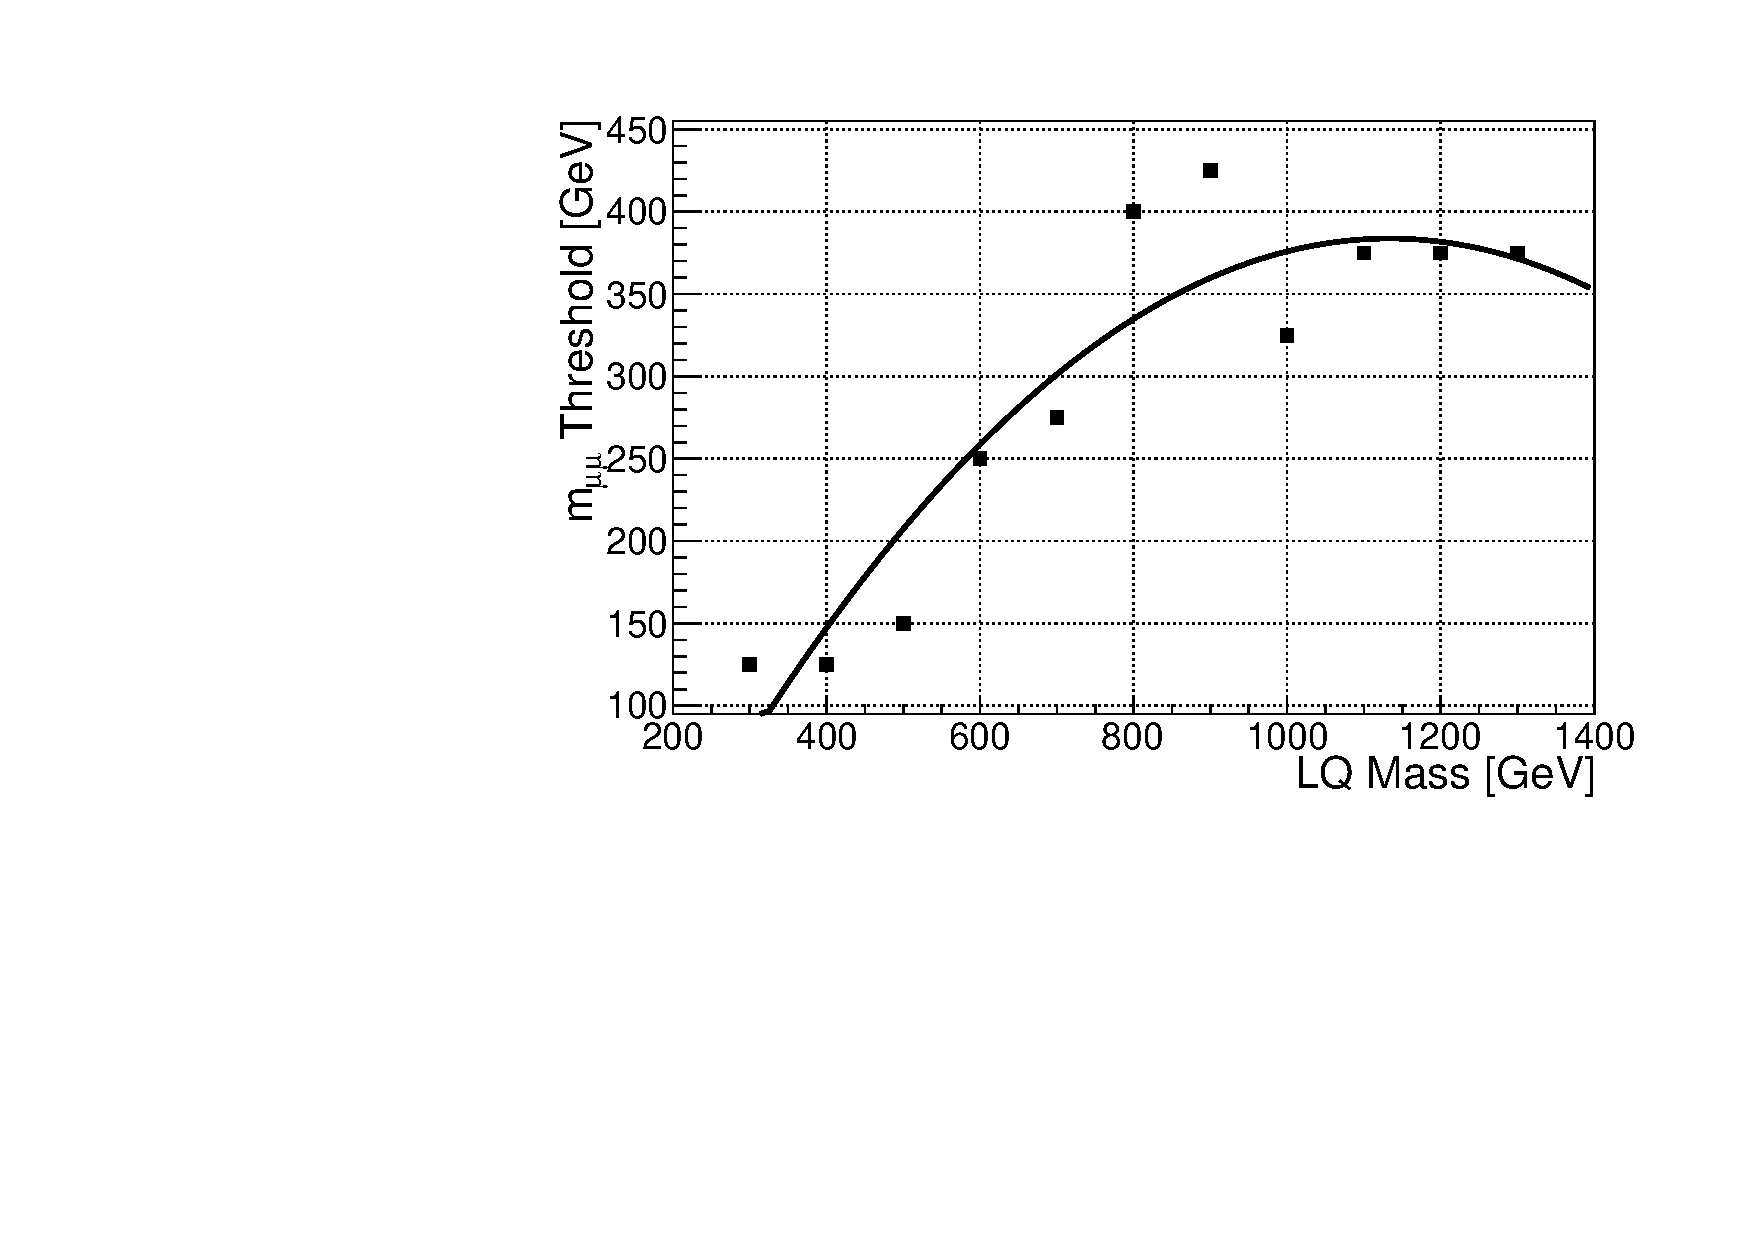
\includegraphics[width=.32\textwidth]{Images/Analysis/Results_Testing_2016_stockNanoAODv6/OptimizationLQ_uujj_M_uu_pol2cutoff.pdf}}
    {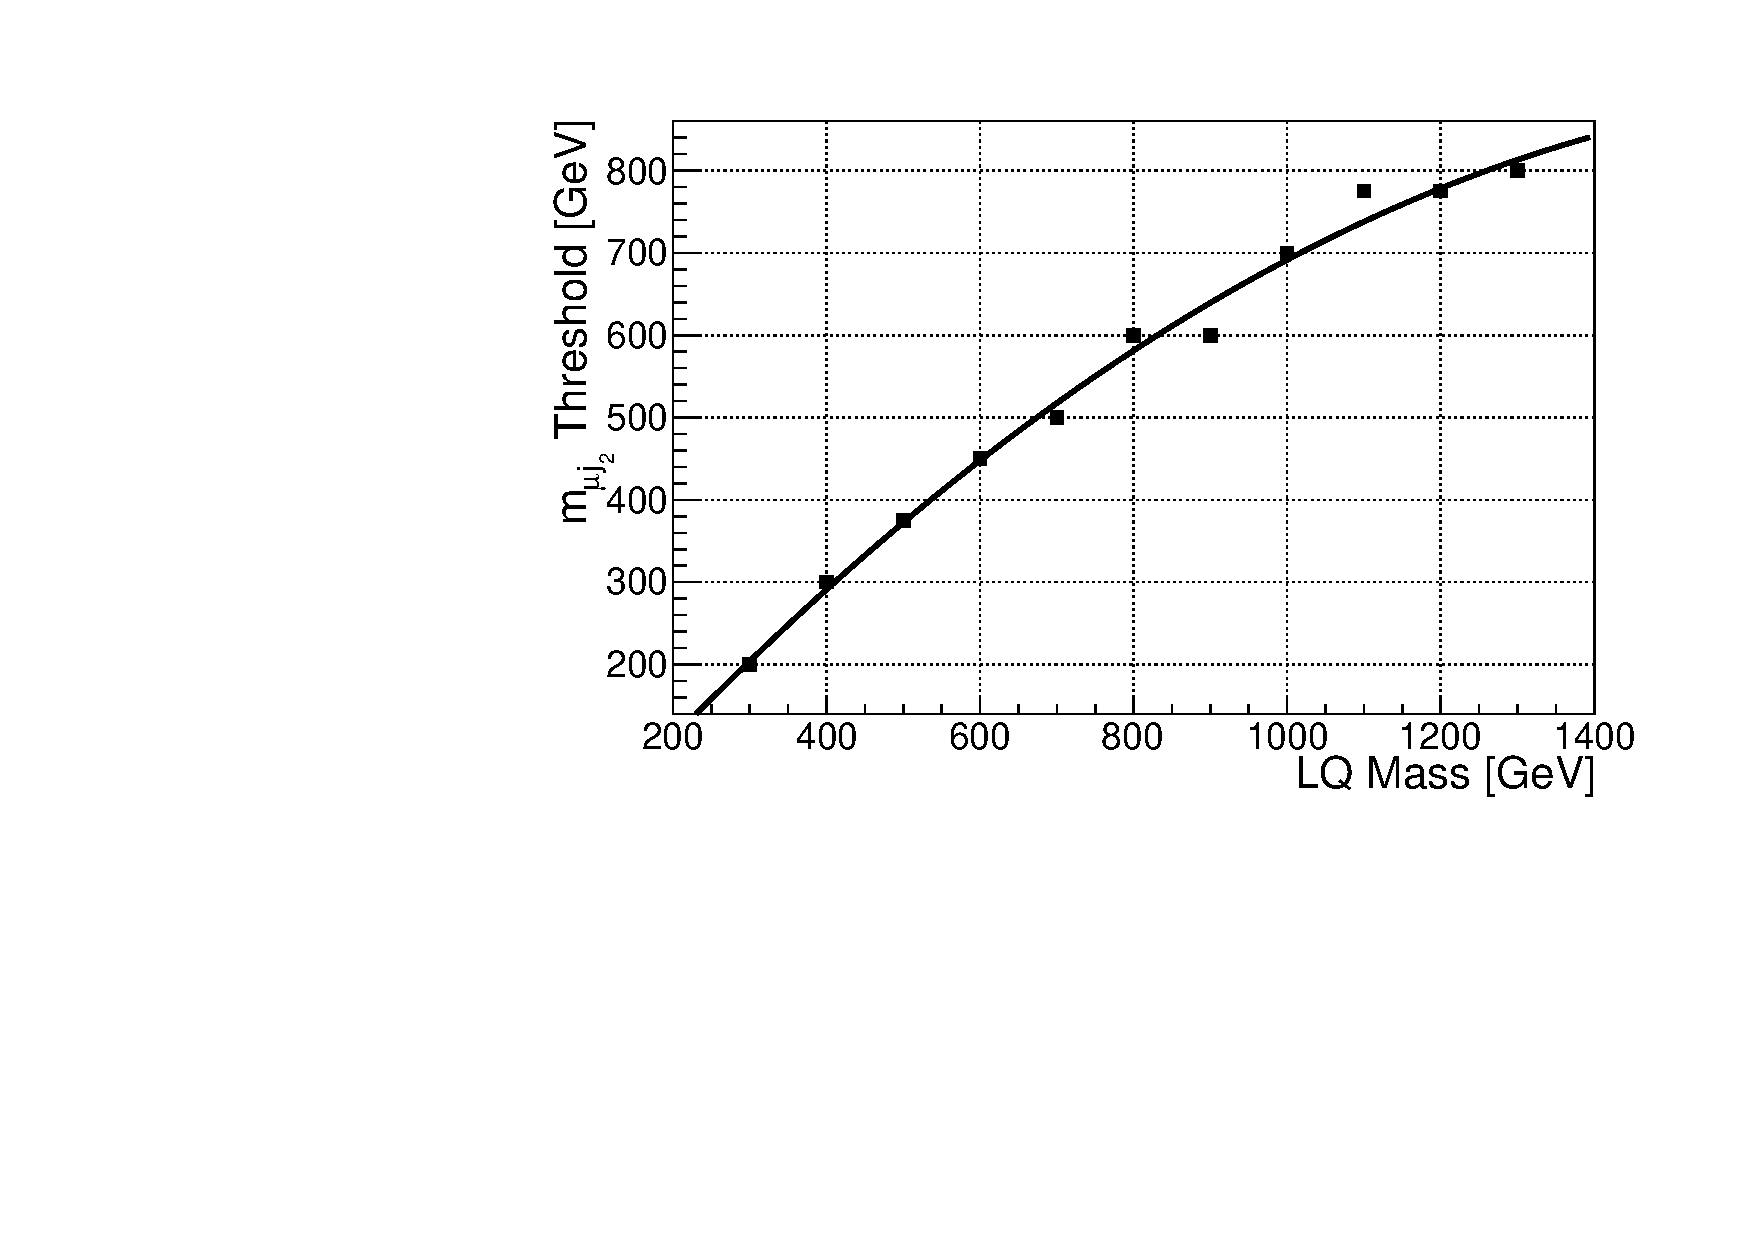
\includegraphics[width=.32\textwidth]{Images/Analysis/Results_Testing_2016_stockNanoAODv6/OptimizationLQ_uujj_M_uujj2_pol2cutoff.pdf}}
    \caption{Top: The optimized thresholds on the variables \ST (left), \Muu (middle), and \MujTwo (right), shown with a quadratic fit of all points. Bottom: The optimized thresholds on the variables \ST (left), \Muu (middle), and \MujTwo (right), up to the cutoff, shown with a quadratic fit of points below the cutoff.}
    \label{figapp:quadraticfits}
\end{figure}

\begin{figure}[H]
    \centering
    {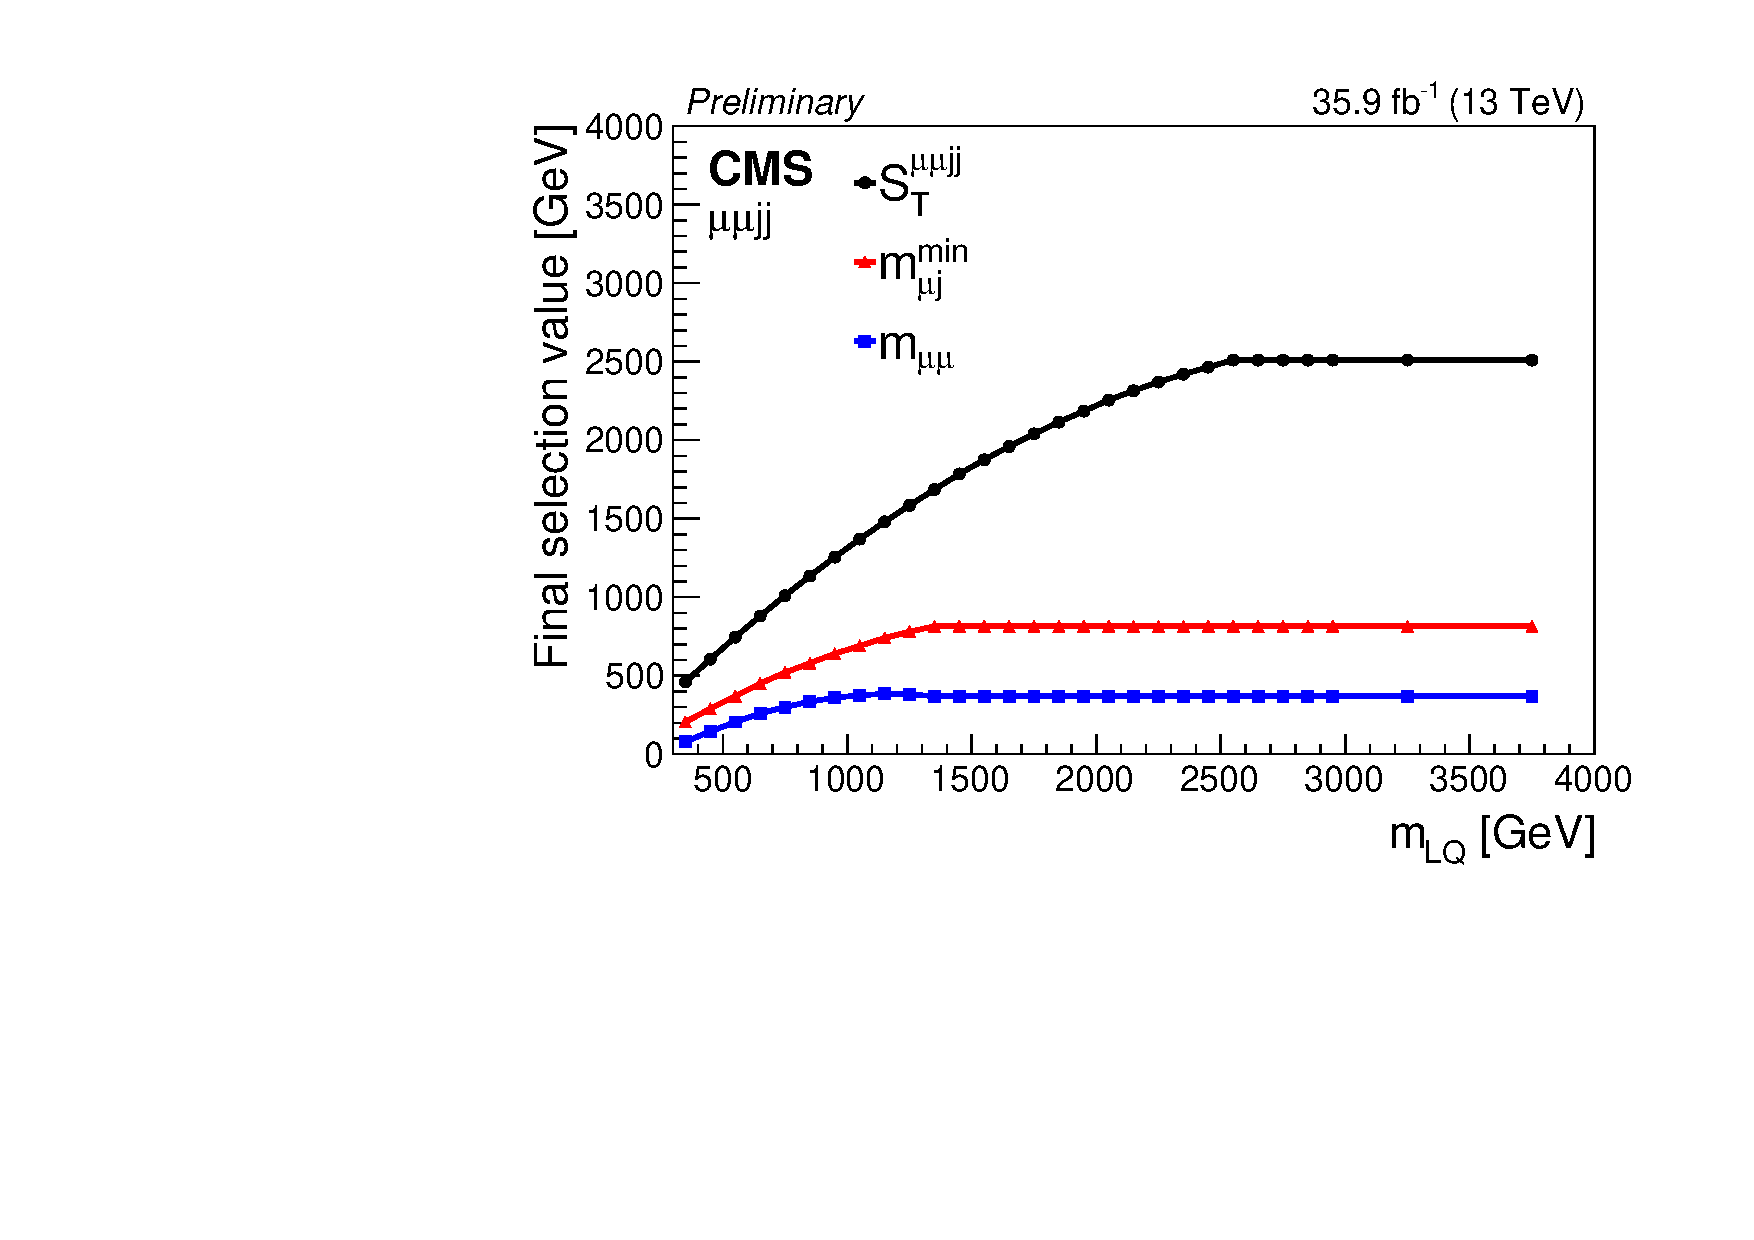
\includegraphics[width=.48\textwidth]{Images/Analysis/Results_Testing_2016_stockNanoAODv6/optPlotuujj_FinalSel.pdf}}
    \caption{The final selection values used in the 3-D optimization study with the variables \Muu, \ST, and \MujTwo as functions of leptoquark mass hypothesis.}
    \label{figapp:3doptimizedcuts}
\end{figure}

The same final selection was used to separate signal from background in all three data-taking years. Expected asymptotic limits at \SI{95}{\%}\CL were placed on the product of the signal production cross-section and branching fraction for the 2016, 2017, and 2018 data-taking years, and for the combined Run 2 dataset, shown in Figs.~\ref{figapp:cutandcountlimits} and~\ref{figapp:cutandcountlimitsrun2}. As systematic uncertainties had not been finalized at the time this study was performed, only statistical uncertainties are included. The expected upper limits place a lower bound on the leptoquark mass of 1650~GeV. Comparing this result with the combined expected lower bound of 1721.2~GeV from the main analysis deminstrates a notable improvement in the use of BDT discriminators over a 3-D optimization. 

\begin{figure}[H]
    \centering
    {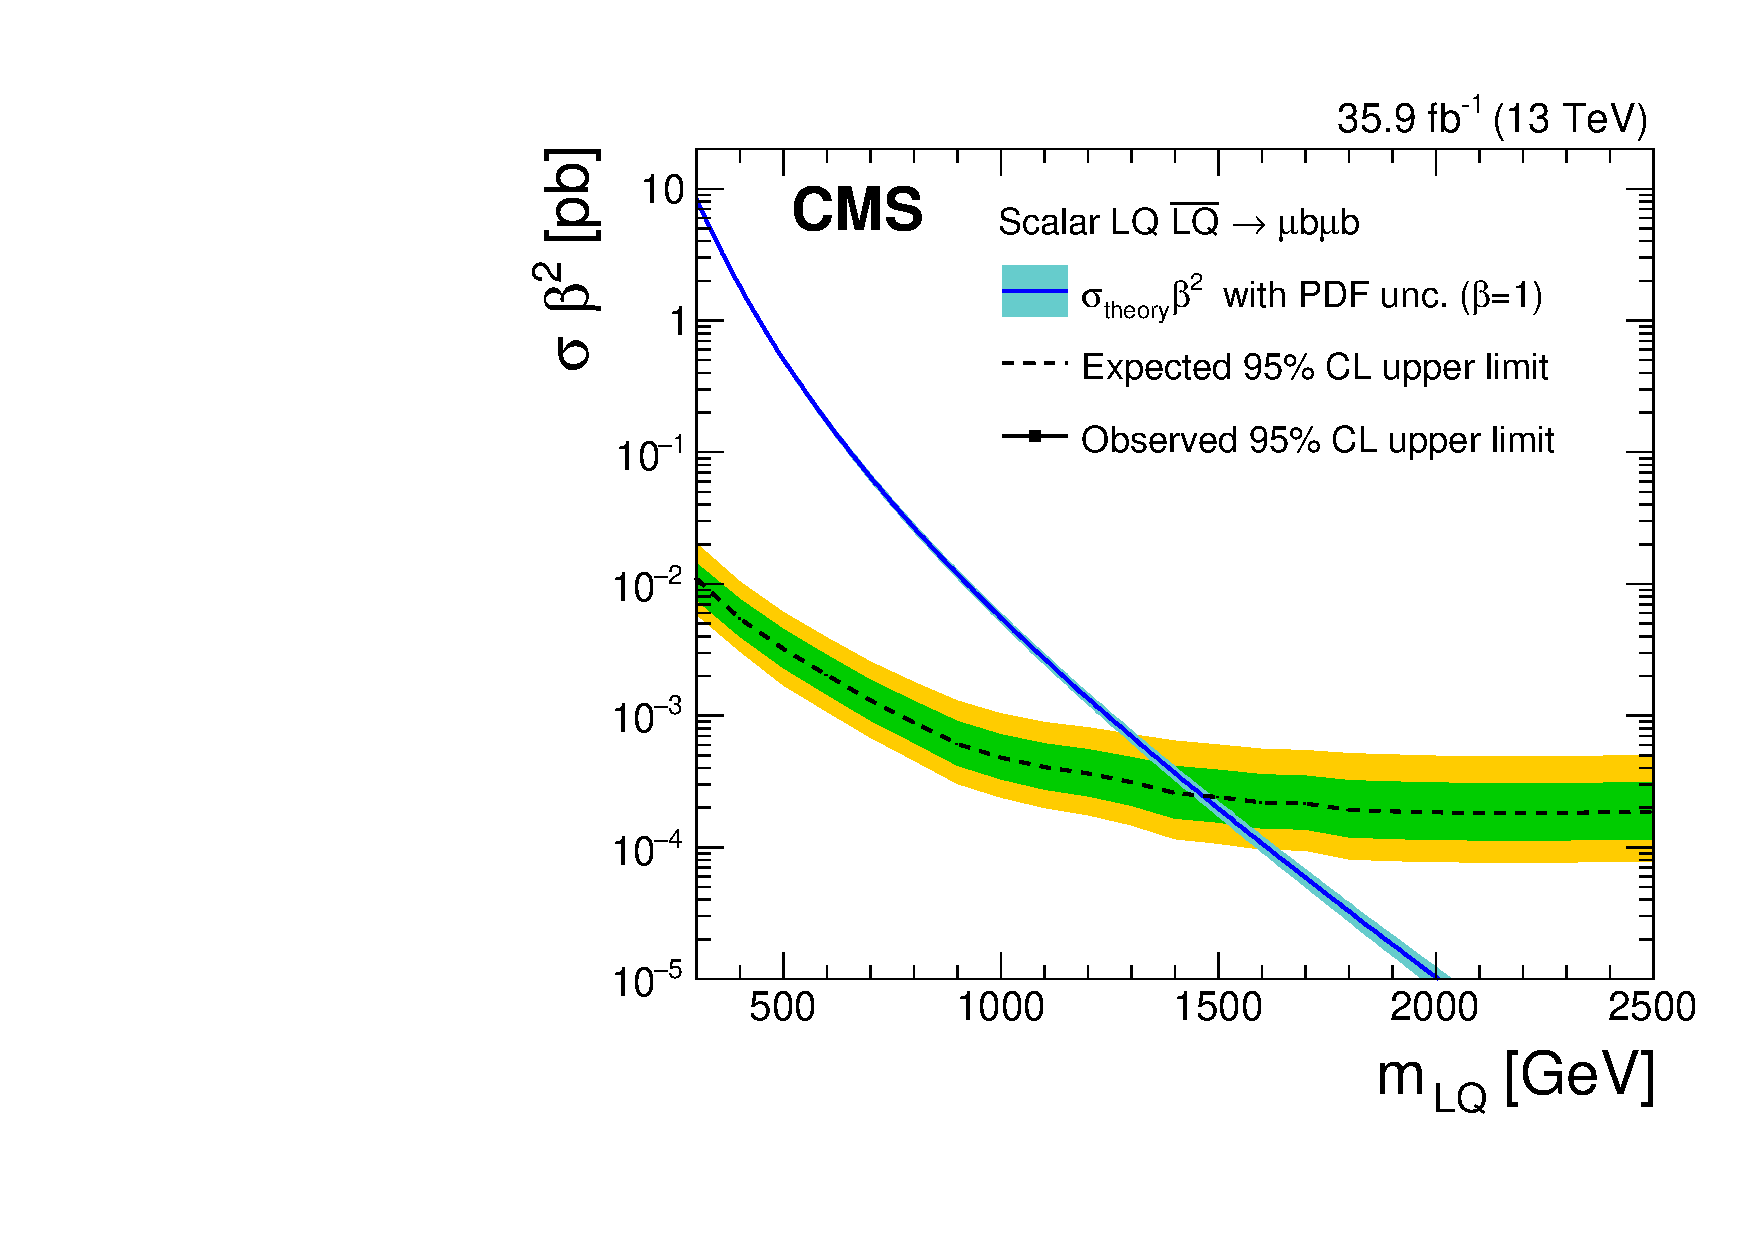
\includegraphics[width=.32\textwidth]{Images/Analysis/3D_Opt_Limits/BR_Sigma_MuMu_2016.pdf}}
    {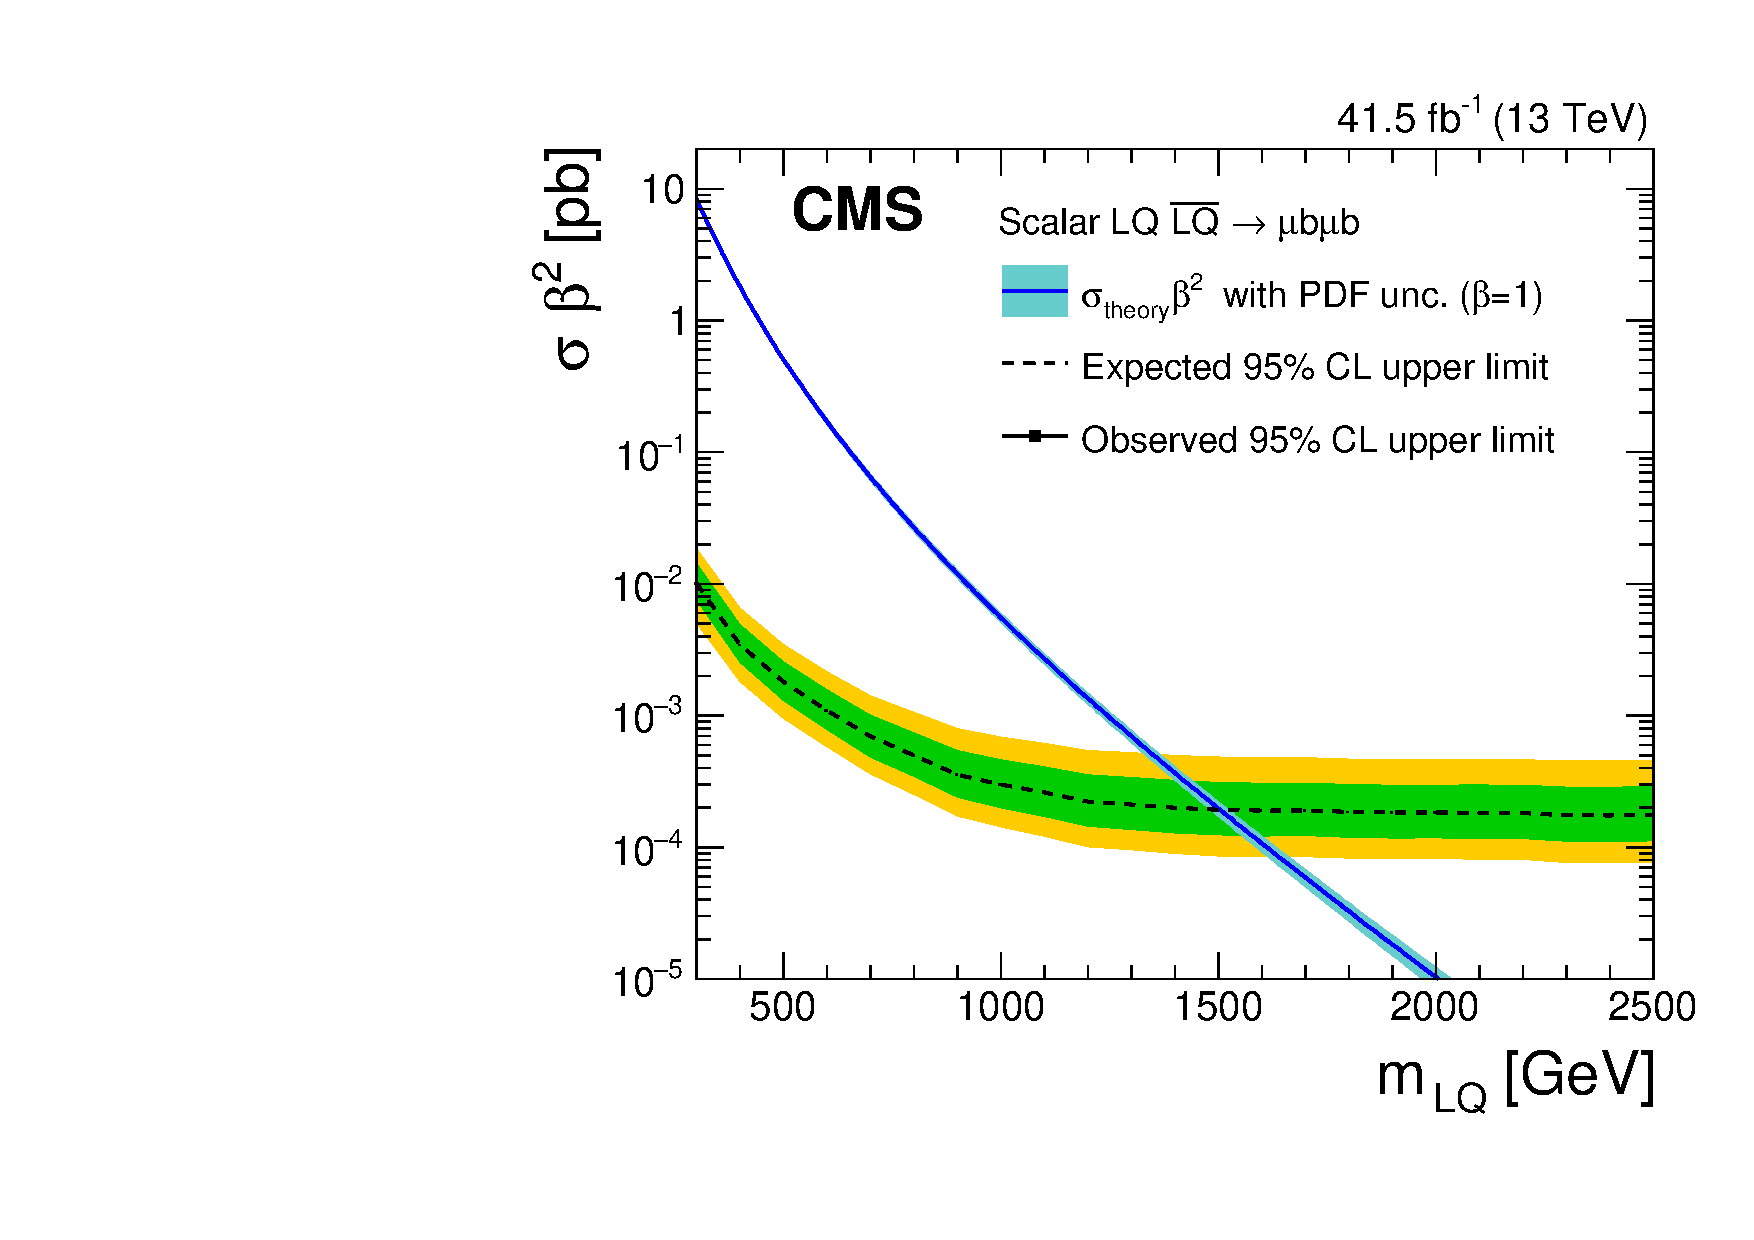
\includegraphics[width=.32\textwidth]{Images/Analysis/3D_Opt_Limits/BR_Sigma_MuMu_2017.pdf}}
    {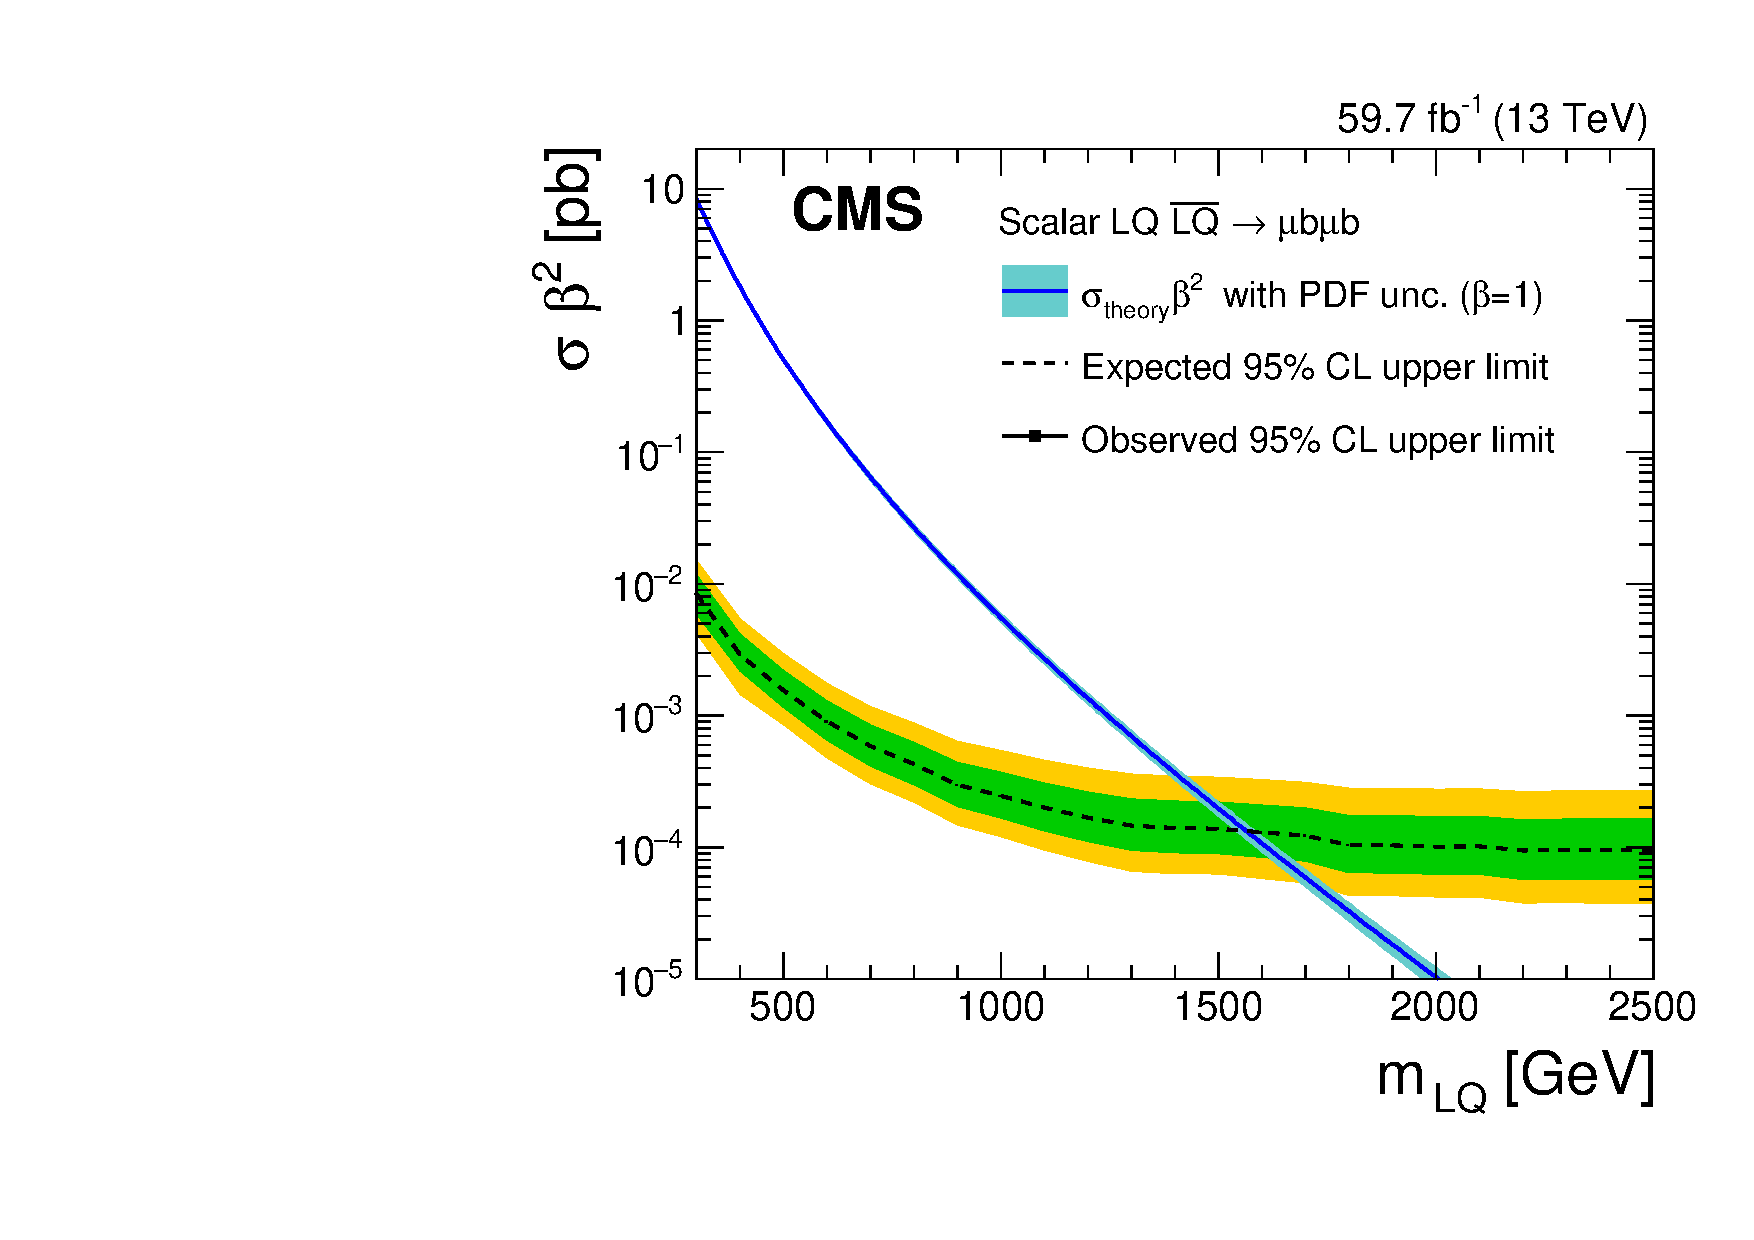
\includegraphics[width=.32\textwidth]{Images/Analysis/3D_Opt_Limits/BR_Sigma_MuMu_2018.pdf}}
    \caption{The expected asymptotic upper limits at \SI{95}{\%} \CL on the leptoquark pair production cross section times squared branching fraction as a function of leptoquark mass obtained from the 3-D optimization study with 2016 (left), 2017 (middle), and 2018 (right) datasets. The expected limits and uncertainty bands represent the median expected limits and the \SI{68}{\%} and \SI{95}{\%} confidence intervals. The \xsecTheory curves and their bands represent, respectively, the theoretical scalar leptoquark pair production cross section and the uncertainties due to the choice of PDF and renormalization/factorization scales.}
    \label{figapp:cutandcountlimits}
\end{figure}

\begin{figure}[H]
    \centering
    {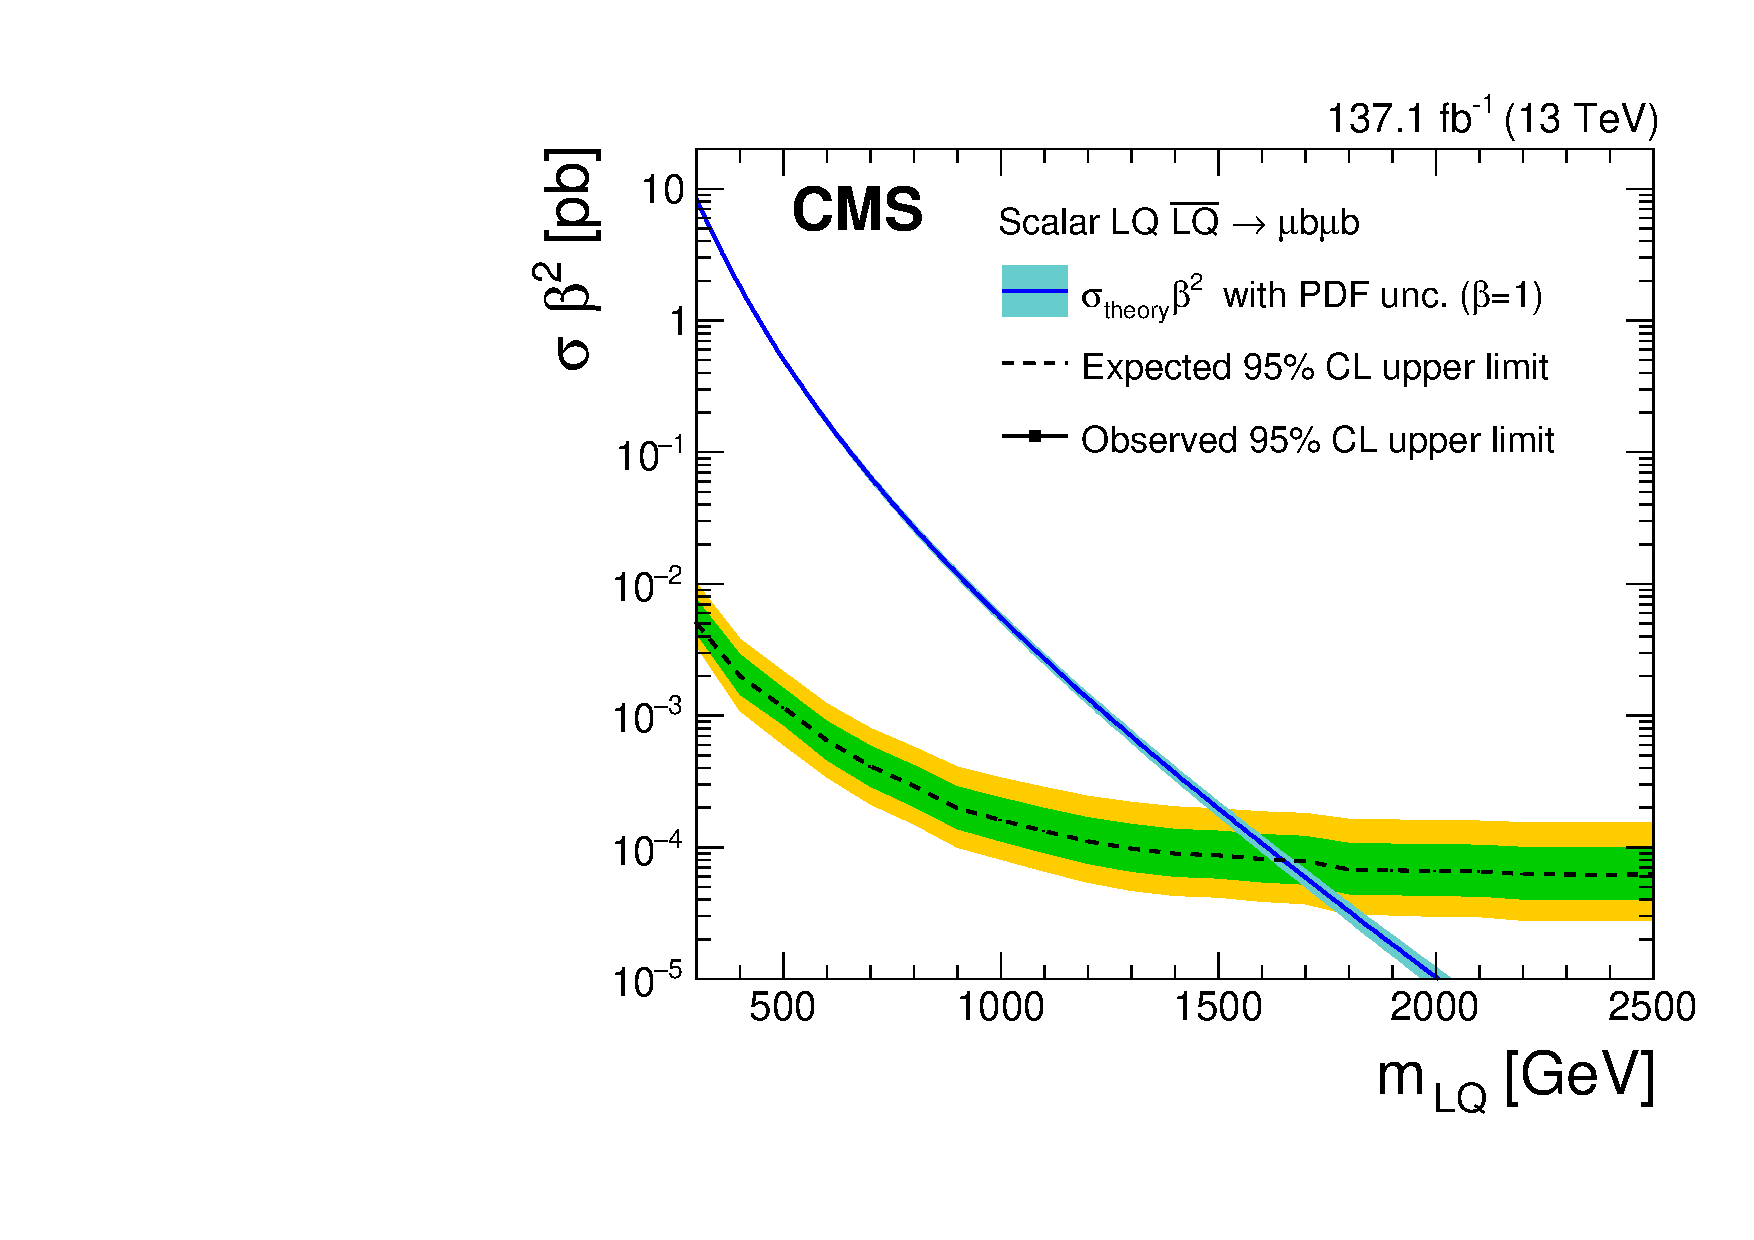
\includegraphics[width=.48\textwidth]{Images/Analysis/3D_Opt_Limits/BR_Sigma_MuMu_2016-2018.pdf}}
    \caption{The expected asymptotic upper limits at \SI{95}{\%} \CL on the leptoquark pair production cross section times squared branching fraction as a function of leptoquark mass obtained from the 3-D optimization study with the combined Run 2 datasets. The expected limits and uncertainty bands represent the median expected limits and the \SI{68}{\%} and \SI{95}{\%} confidence intervals. The \xsecTheory curves and their bands represent, respectively, the theoretical scalar leptoquark pair production cross section and the uncertainties due to the choice of PDF and renormalization/factorization scales.}
    \label{figapp:cutandcountlimitsrun2}
\end{figure}